\section{Introduction}
\protect\label{section:intro}

\engdate

This report describes steps taken to analyse observational data from the
{\rem} (Rapid Eye Mount) telescope and camera equipment in La Silla, Chile, as
operated by the Red Dots Project. This work commenced in March 2015.
\citep{reddotsspace20}. However the data collection for the project did not
start until mid-July 2017.

The {\rem} telescope has been set up to take a series of automatic
observations of patches of sky on a nearly nightly basis. The main concern of
the Red Dots Project is of {\rdwarf} stars and as the {\rem} observatory is
concurrently used for other projects, for example \citet{giannini18}, this
report focuses on the {\rdwarf} targets designated by the Red Dots Project,
which started in mid-2017. All observations ceased on March 2020 due to the
Coronavirus pandemic but were restarted in October 2020 and continued up until April 2022.

The original objectives of the work documented in this report are:
\begin{enumerate}
  \item To set up a pipeline for automatic analysis and processing of the data.
  \item To evaluate to what degree reliable photometry, together with an
  estimate of the error bars, can be obtained in relation to the targets of
  interest.
  \item If accuracy and reliability of the photometry permit, obtain periodic
  data for the target stars of particular interest.
\end{enumerate}

Other supplementary objectives came to light over the course of the work. An
early example of this was obtaining a rotation period for \ross. As noted in
Section \ref{section:targets}, there is a little lack of clarity and some
contradictions in the published rotation period, so I undertook some work to establish the rotation period of {\ross}
from existing data sources and then attempt to recover the same period from the {\rem} data.

\subsection{The {\rem} telescope}
\protect\label{section:remscope}

The {\rem} observatory at La Silla was initially set up in 2003
\citep{antonelli05} consisting of the the REMIR near-infrared camera and the
visible light camera, ROSS, which was upgraded in 2015 to the ROSS2 camera.

Light to the REMIR telescope is split between 3 filters, \texttt{H}, \texttt{J}
and \texttt{K} with one of seven of dither patterns. Images are returned as
512x512 arrays with reduction already carried out using PREPROCESS software
\citep{dipaola01}, as described in \citet{calzoletti05}. The REMIR observations
were discontinued at the beginning of June 2019 due to a system fault. They were
restarted at the beginning of February 2021.

The visible light portion of the light from the telescope is split between 4
Sloan-style filters and projected onto quadrants of a 2048x2048 CCD array, which
is an ANDOR Ikon-L series chip. The names, quadrants and bandwidths of the 4
filters are set out in Table \ref{table:ros2quad}.

\begin{table}[!htbp]
\begin{center}
\begin{tabular}{llrr} \hline
Filter & Quadrant & Low bw (nm) & High bw (nm) \\\hline
\texttt{g'} & Upper Right & 400 & 550 \\
\texttt{r'} & Lower Right & 550 & 700 \\
\texttt{i'} & Upper Left & 700 & 820 \\
\texttt{z'} & Lower Left & 820 & 1000 \\
\hline
\end{tabular}
\end{center}
\caption{The four ROSS2 filters, quadrant used on the CCD chip, low and high
bandwidth in nm. Hereinafter the filters are referred to as \texttt{g},
\texttt{r}, \texttt{i} and \texttt{z} respectively and the quadrants as UR, LR,
UL and LL.} \protect\label{table:ros2quad}
\end{table}

The images from the visible light telescope are nominally 1024 by 1924 pixels,
although the effective area is only in the region of 900 by 900
pixels varying for each filter as the settings are periodically adjusted.
As a consequence of the construction of the ROSS2 camera, all of the visible
light images are taken at exactly the same time with exactly the same
exposure, viewing exactly the same patch of sky. In Fig. \ref{fig:showusedccd}
is shown the areas on the CCD used by various filters at various times.

\begin{figure}[!htbp]
\begin{center}
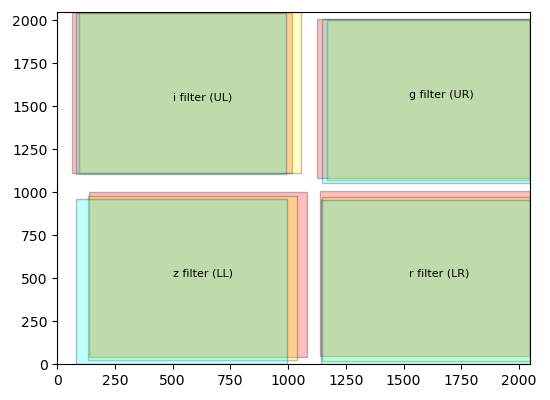
\includegraphics[scale=1]{images/showusedccd.png} \\
\end{center}
\caption{This figure sets out the areas of the CCD used by the ROSS2
telescope which are used for the various filters at various times after
adjustment of the telescope. The area shaded in red is that prior to July 2015, the yellow shaded area is between
then and March 2019 and the blue part after then. The bulk of the area is
common to all of the configurations as can be seen. Note that all of the
{\rdwarf} observations, with which this report is concerned, start in 2017, well
after the first reconfiguration.} \protect\label{fig:showusedccd}
\end{figure}

Bias frames are taken daily for the visible light filters, usually 5 at
approximately 11:30 am and flat field frames nearly as often, usually 3 at a
time as the sky fades. A monthly master flat and bias file for each visible
light filter is also constructed from the daily flat and bias frames.

\subsection{Targets}
\protect\label{section:targets}

The three main targets of the Red Dots REM observations are \prox, {\bstar} and
\ross, all \rdwarf s.

\begin{description}
\item[\prox] is of spectral type M5.5 and at 1.30197 pc. is the nearest known
stellar object to the solar system. It is noted as having a significant flare activity, calculated
at 1.49 events per day in \citet{vida19} despite having a slow rotation period,
calculated at at 82.6 $\pm$ 0.1 days in \citet{collins17}.
\item[\bstar] is of spectral type M4 and at 1.8282 pc, is the fourth closest
stellar object to the solar system after {\prox} and Alpha Centauri A and B. Its
rotation period has been progressively given as 130 days in \citet{benedict98},
148.6 days in \citet{suarezmascareno15} and 145 $\pm$ 15 days in \citet{toledopadron18}.
Activity is low, as noted in the latter.
\item[\ross] is of spectral type M3.5 and at 2.976 pc, is the eleventh nearest
known stellar object to the solar system. Its strong activity is noted in
\citet{wargelin08}. As discussed in the draft paper included herewith, there is a wide variation in
some of the parameters for {\ross}, in particular the value of \vsini, the
radius and the rotation period. It became clear that an early benchmark of the work on the
{\rem} data would be clarification of the rotation period.
\end{description}

\subsection{Number of observations}
\protect\label{section:numobs}

The number of observations for each of the targets (and other objects used in
other projects) is given in Table \ref{table:numobs}. In Fig.
\ref{fig:rdwarfhist} is shown the distribution of observations of these targets
by date.

\begin{table}[!htbp]
\begin{center}
\begin{tabular}{lrr}
Target & Number of obs & \% \\
\hline
\prox & 36,312 & 17.16 \\
\bstar & 8,785 & 4.15 \\
\ross & 23,236 & 10.98 \\
Others & 143,329 & 67.72 \\
\hline
Total & 211,662 \\
\end{tabular}
\end{center}
\caption{This table shows the number of observations taken of each target
object, also showing the number of observations of other objects taken by other
projects. The number of usable observations of each target object is roughly
94\%
for the {\gfilter} and {\rfilter} cases, but significantly more for the
{\ifilter} and {\zfilter} cases.} \protect\label{table:numobs}
\end{table}

\begin{figure}[!htbp]
\begin{center}
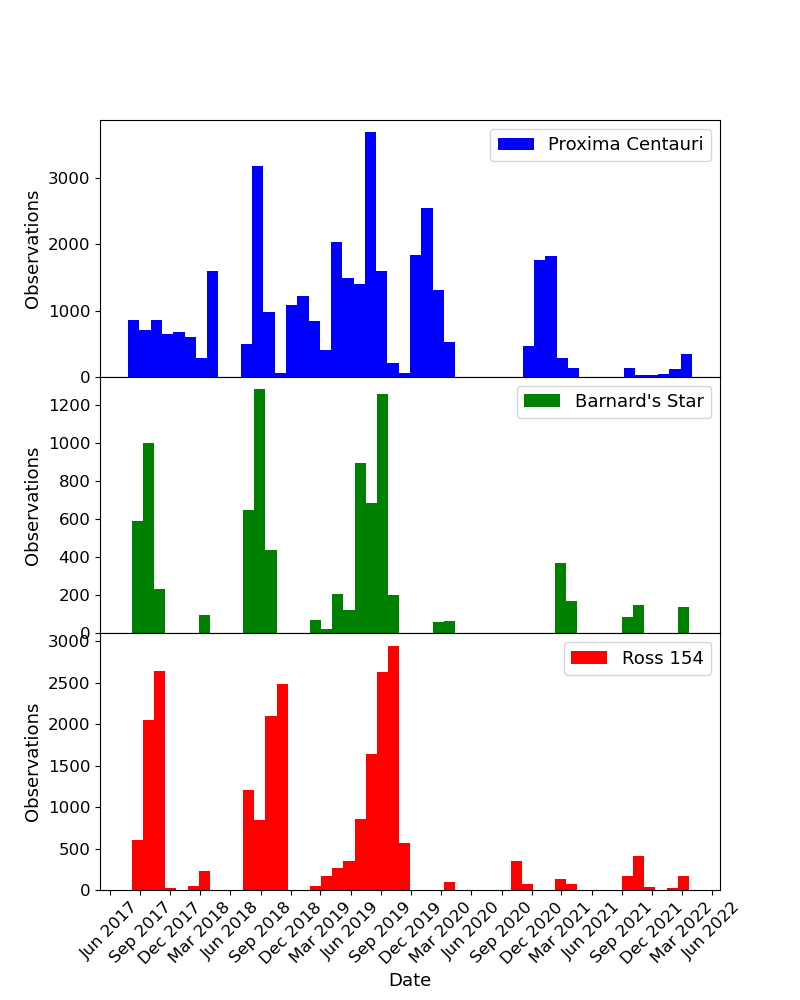
\includegraphics[scale=0.60]{images/rdwarfhist.png} \\
\end{center}
\caption{This figure shows the distribution of observations of the three
{\rdwarf} targets to date, with {\prox} observations in the top pane, {\bstar}
in the middle pane and {\ross} in the bottom pane.}
\protect\label{fig:rdwarfhist}
\end{figure}

\subsection{Rotation periods and activity}
\protect\label{section:rotact}

The rotation period of each of the targets represents a most obvious
first objective of this study. As discussed in the draft paper, it is clear that
any surface features of the star, light or dark, cause a periodic signal to be
observed corresponding to the rotation period.

Rotation periods can give an indication of the age of the star, as discussed,
for example in the case of \ross, in \citet{wargelin08}. It has also been
noticed that a fast rotation period is correlated with strong activity. In
\citet{mohanty03} it is seen how activity increases, up to a limit, with a fast
rotation period. There have been various other studies, for example
\citet{aizawa22} and \citet{magaudda22} are recent papers in which rotation
periods and activity cycles are studied.

For this reason I decided to use detection of the rotation period as a benchmark
for analysis of the {\rem} data. The rotation period of {\ross} was somewhat
unclear in the literature and I made an effort to extract it from the data the
other literature referred to and then from the {\rem} data. Various figures for
the rotation period of {\bstar} exist and this is a clear target for further
study, however it should be noted that there are rather less observations of
\bstar, as noted in Section \ref{section:numobs}. Hopefully it may be possible
to obtain information about activity cycles and add to the correlation of this
with the rotation period.

\subsection{Proper Motions and caveats}
\protect\label{section:propermotions}
As all the target objects are amongst the closest objects outside the solar
system, they all have particularly large proper motions. Care must be taken to
track the proper motions of the targets and any adjacent objects.

The resolution of the ROSS2 camera is such that successive pixels
are approximately 0.6 arc-seconds apart (about 4.9 for Declination values, 6.9
for Right Ascension values but that varies a little with declination). This
means that proper motions of less than 20 milliarcseconds per year may be safely
disregarded which eliminates all but a handful of objects\footnote{18 objects
altogether, 10 in the vicinity of \prox, 1 in the vicinity of {\bstar} and 7 in
the vicinity of \ross.} in the vicinity of the targets from a need to track proper
motions for the bulk of other objects.

In Fig. \ref{fig:proxpm}, Fig. \ref{fig:bspm} and Fig. \ref{fig:rosspm} are
illustrated the proper motions \prox, {\bstar} and {\ross} respectively against
the immediate backgrounds.

\begin{figure}[!htbp]
\begin{center}
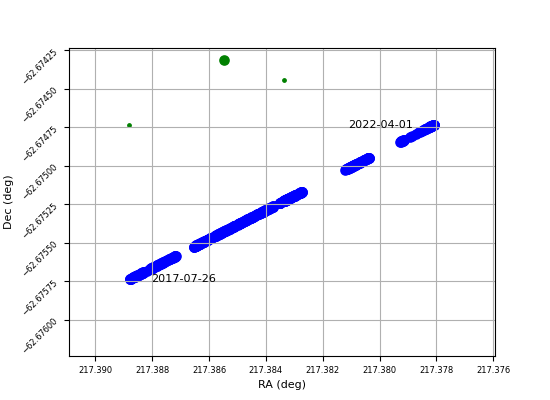
\includegraphics[scale=0.7]{images/pmprox.png} \\
\end{center}
\caption{This figure tracks the proper motion of {\prox} against the immediate
background stars, showing start and end dates of the observations at the time
of writing, the gaps showing the periods where observations were not taken.
The relative sizes of the objects, including \prox, are based on the selected
apertures determined from subsequent processing.} \protect\label{fig:proxpm}
\end{figure}

\begin{figure}[!htbp]
\begin{center}
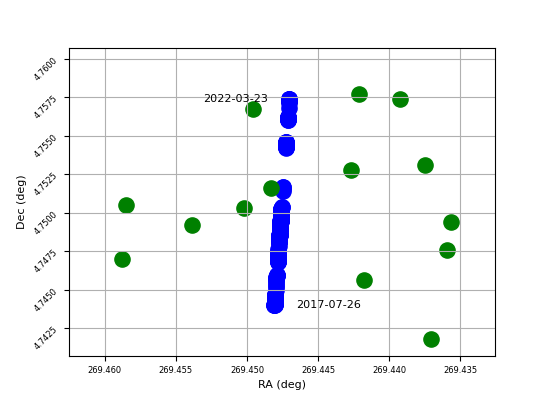
\includegraphics[scale=.8]{images/pmbstar.png} \\
\end{center}
\caption{This figure tracks the proper motion of {\bstar} against the immediate
background stars, showing start and end dates of the observations at the time
of writing, the gaps showing the periods where observations were not taken. The proper motion of {\bstar} is
extremely large and the scale is not the same as in Fig. \ref{fig:proxpm} or
Fig.  \ref{fig:rosspm} in consequence. Proper motion on Declination is so large
that the scale is reduced by a factor of 10 from that in Right Ascension.
Again relative sizes of the objects reflect those of the objects in the images,
including \bstar.} \protect\label{fig:bspm}
\end{figure}

\begin{figure}[!htbp]
\begin{center}
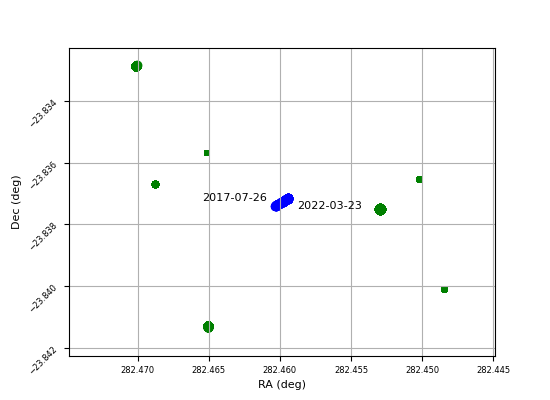
\includegraphics[scale=0.7]{images/pmross.png} \\
\end{center}
\caption{This figure tracks the proper motion of {\ross} against the immediate
background stars, showing start and end dates of the observations at the time
of writing, the gaps showing the periods where observations were not taken.
The scale is the same as in Fig. \ref{fig:proxpm} (but not the same as in Fig.
\ref{fig:bspm}). Again relative sizes of the objects reflect those of the
objects in the images.} \protect\label{fig:rosspm}
\end{figure}

\clearpage
